\begin{figure}[ht]\centering
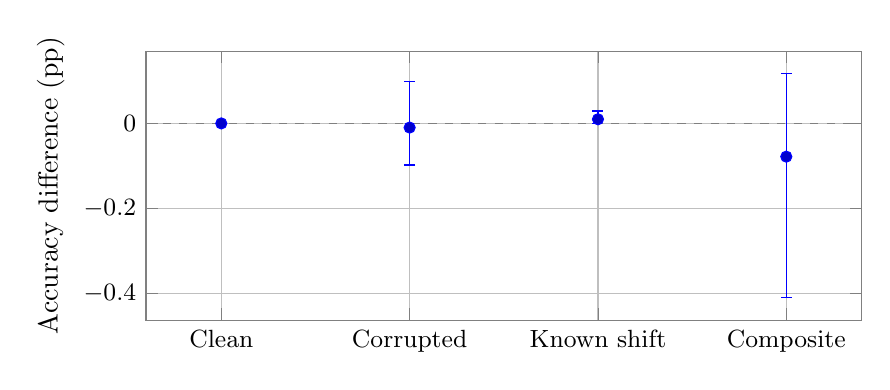
\begin{tikzpicture}\begin{axis}[width=.88\linewidth,height=5cm,
ylabel={Accuracy difference (pp)},xtick={0,1,2,3},
xticklabels={Clean,Corrupted,Known shift,Composite},xmin=-.4,xmax=3.4,
grid=major,axis line style={gray},tick label style={font=\small}]
\addplot+[only marks,mark=*,error bars/.cd,y dir=both,y explicit] coordinates {
(0,0.0) += (0,0.0) -= (0,0.0)
(1,-0.009765625) += (0,0.10742187500000001) -= (0,0.087890625)
(2,0.009765625) += (0,0.01953125) -= (0,0.009765625)
(3,-0.078125) += (0,0.1953125) -= (0,0.33203125000000006)};
\addplot[dashed,gray,domain=-.4:3.4] {0};
\end{axis}\end{tikzpicture}
\caption{Adaptive robust minus the development-selected control. Error bars
show descriptive 95\% paired dataset-cluster bootstrap intervals. Only the
composite contrast is the improvement primary; its practical threshold is +2 pp.}
\end{figure}
